\documentclass[journal]{IEEEtran}
\usepackage{newtxtext,newtxmath}
\IEEEoverridecommandlockouts

\usepackage{amsmath,amsfonts}
\usepackage{listings}
\usepackage{graphicx}
\usepackage{hyperref}
\usepackage{url}
\usepackage{xcolor}
\usepackage{caption}

\lstset{
  basicstyle=\ttfamily\small,
  breaklines=true,
  frame=single,
  columns=fullflexible,
  keepspaces=true,
  showstringspaces=false
}

\title{A Context-Aware Ensemble Learning Framework for Vulnerability Prioritization in Critical Infrastructure}

\author{%
  \IEEEauthorblockN{Harshavardhan Malla}
  \IEEEauthorblockA{Independent Researcher\\ Email: harshavardhanmalla75@gmail.com}%
}

\renewcommand{\textendash}{-}
\renewcommand{\textemdash}{-}
\usepackage{xurl}
\usepackage{etoolbox}
\makeatletter
\patchcmd{\abstract}{---}{:\space}{}{}
\patchcmd{\IEEEkeywords}{---}{:\space}{}{}
\makeatother
\begin{document}
\maketitle

\begin{abstract}
This study introduces a context-aware machine learning framework for vulnerability prioritization in critical infrastructure. While current practices rely on static metrics such as CVSS, they lack environmental context and exploitability signal. We propose an ensemble of Random Forest and XGBoost that fuses vulnerability metadata, threat-intelligence indicators (KEV membership, public proof-of-concept, ATT\&CK mapping), and environmental context (asset criticality, exposure, patch age, vulnerability density). To support reproducibility, we evaluate on a pre-registered synthetic benchmark that models 18 monthly Patch Tuesday cycles across a 50,000-endpoint government fleet, with all code and frozen results released. Across 25 seeds, the ensemble attains a Precision@50 of 0.74 against 0.22 for CVSS-only ranking, lowers the high-risk miss rate from 0.67 to 0.18, and raises within-window SLA compliance from 0.64 to 0.98; under a capacity-constrained remediation scheduler it cuts mean time to remediate by 62\% (6.2 to 2.3 days). Every gain is supported by a pre-registered hypothesis whose bias-corrected and accelerated bootstrap interval excludes zero. The framework integrates with SCCM and Intune patch workflows, giving a scalable, audit-ready, context-sensitive approach to patch prioritization in regulated environments.
\end{abstract}

\begin{IEEEkeywords}
Patch Tuesday, machine learning-based prioritization, CVE, critical infrastructure, threat intelligence integration, Random Forest, XGBoost, vulnerability management automation
\end{IEEEkeywords}

\section{Introduction}

In the contemporary cybersecurity environment, prompt vulnerability management is an essential duty, especially in sectors such as government, utilities, transportation, and defense. Despite progress in vulnerability scoring, a gap remains in real-time, contextual prioritization that incorporates live exploit intelligence, asset significance, and compliance timelines directly into operational patch workflows. Microsoft's ``Patch Tuesday,'' a monthly scheduled delivery of security patches, has become a critical event in enterprise IT calendars \cite{ms_patchtuesday}. The predictability provides operational planning benefits, but it also creates a concentrated period during which numerous Common Vulnerabilities and Exposures (CVEs) must be rapidly studied, tested, and deployed. The risks are particularly elevated in critical infrastructure settings, where even temporary exposure to an actively exploited vulnerability can result in severe operational, financial, and reputational consequences.

Historically, vulnerability prioritization in corporate settings has depended on the Common Vulnerability Scoring System (CVSS) \cite{cvss}, which offers a standardized numerical severity assessment for each CVE. Although CVSS provides a valuable foundation, it is fundamentally static and lacks contextual relevance. It fails to account for real-time exploitability, the availability of public proof-of-concept (PoC) code, or the particular criticality of the assets at stake \cite{bozorgi2010,sabottke2015}. Existing governmental and enterprise procedures often exhibit insufficient machine learning integration within tools like SCCM and Intune, leading to delays between threat detection and remediation. This disparity frequently results in skewed remedial priorities: high-scoring vulnerabilities that are unlikely to be exploited may receive resources over lower-scoring but actively weaponized threats. In government contexts, these inefficiencies not only elevate risk but also impede the patch management process as a whole.

The complexity of the challenge is amplified by operational limitations, including restricted maintenance periods, strict compliance mandates (CJIS, NIST, FedRAMP) \cite{nist_800_40,nist_800_53,fedramp}, and the diversity of endpoints distributed across several regions and administrative domains. Manual triage methods are inadequate for environments with tens of thousands of devices, while fully automated systems lacking contextual intelligence may overwhelm teams with false positives. These constraints highlight the need for a context-sensitive and scalable prioritization system that can be seamlessly integrated into existing patch deployment processes.

This study introduces a machine learning-based predictive prioritization framework aimed at improving Patch Tuesday operations inside critical infrastructure environments. Our solution integrates multiple data sources-National Vulnerability Database (NVD) entries \cite{nvd}, CISA Known Exploited Vulnerabilities (KEV) catalog \cite{cisa_kev}, exploit database records \cite{exploitdb}, MITRE ATT\&CK mappings \cite{mitre_attack}, and enterprise telemetry from SCCM, Intune, and Tanium \cite{tanium}-to compute a dynamic risk score for each CVE. This score combines technical severity and environmental context, enabling more accurate identification of high-impact vulnerabilities. The framework also includes a Group Policy Object (GPO)-agnostic PowerShell automation for background updating of AppX packages without requiring policy modifications. The goal is to convert Patch Tuesday from a reactive operational burden into a proactive, intelligence-assisted security workflow.

\section{Background}

Patch management is a foundational element of an organization's cybersecurity strategy. The phrase ``Patch Tuesday'' derives from Microsoft's routine of issuing security patches on the second Tuesday of each month \cite{ms_patchtuesday}, a practice initiated in October 2003. Originally designed to provide predictability for IT teams, Patch Tuesday has evolved into a global cybersecurity event, with vendors, analysts, and adversaries all anticipating the publication of new vulnerabilities and fixes. Critical infrastructure operators face heightened stakes, as these environments frequently underpin essential public services, including transportation systems, energy grids, and law enforcement networks. A single missed or delayed patch can create significant risk exposure.

The complexity of patch management in these environments is substantial. Large corporations and governmental organizations frequently manage tens of thousands of diverse endpoints across multiple Windows versions, server roles, and application frameworks. These endpoints may be geographically dispersed, connected through varied network conditions, and subject to strict uptime requirements. Implementing fixes without disrupting mission-critical services requires careful planning, phased rollouts, and extensive testing. The publication of numerous CVEs on Patch Tuesday creates an immediate triage problem, since security teams must determine which vulnerabilities require urgent treatment and which may be deferred without creating unacceptable risk.

Government agencies and regulated industries face additional challenges from a compliance standpoint. Frameworks such as the Criminal Justice Information Services (CJIS) Security Policy, the National Institute of Standards and Technology (NIST) Special Publication 800-53 \cite{nist_800_53,nist_800_40}, and the Federal Risk and Authorization Management Program (FedRAMP) impose strict timelines for remediating high-severity vulnerabilities \cite{fedramp}. Non-compliance may lead to audit findings, revocation of authorization, or financial penalties. The urgency imposed by compliance exacerbates the difficulty of reconciling security requirements with operational realities, especially when patching may affect mission-critical applications or systems.

The shifting threat landscape further intensifies these difficulties. Adversaries have adapted to the Patch Tuesday routine, often reverse-engineering released fixes to create exploits within hours or even minutes of disclosure. In recent years, zero-day vulnerabilities addressed on Patch Tuesday have been followed quickly by broad exploitation campaigns, emphasizing the need for rapid prioritization and deployment. In this setting, depending exclusively on static CVSS ratings for triage is insufficient. A contemporary, context-sensitive methodology is needed-one that integrates real-time exploit intelligence, asset exposure, and organizational impact into a unified prioritization framework. That requirement motivates the machine learning-based approach presented in this study.

\section{Related Work}

Vulnerability prioritization is a dynamic field of research and industrial development, especially as organizations contend with the growing number of published CVEs and the shrinking interval between disclosure and exploitation \cite{cvss}. This section reviews relevant literature and operational methodologies, grouped into conventional severity-based procedures, machine learning-enhanced strategies, and integrated commercial solutions.

\subsection{Severity-Based and Manual Prioritization Approaches}

The most common approach for prioritizing patches is the use of the Common Vulnerability Scoring System (CVSS), which assigns a standardized numeric score derived from metrics such as attack vector, attack complexity, required privileges, user interaction, and the effects on confidentiality, integrity, and availability. While CVSS provides a common severity metric, it is fundamentally static and cannot adapt to evolving threat conditions. Many organizations supplement CVSS scores with internal risk assessments, often conducted manually by security analysts who evaluate factors such as asset criticality, system exposure, and operational significance. This manual triage process may achieve reasonable accuracy in small environments but does not scale efficiently in enterprise infrastructures containing tens of thousands of endpoints. Moreover, the delay introduced by human evaluation can leave important systems exposed during high-risk intervals, particularly immediately after Patch Tuesday.

\subsection{Machine Learning in Vulnerability Prioritization}

Scholarly work has explored the use of machine learning methods in vulnerability management. Models such as VulnPredict and CVE-BERT apply natural language processing (NLP) to CVE descriptions and associated security bulletins to predict exploitability or categorize vulnerabilities into urgency classes \cite{vulnpredict,cvebert}. Other studies have proposed supervised learning frameworks that combine CVSS vectors with threat intelligence signals to produce a composite risk score. For example, prior research has incorporated exploit proof-of-concept availability \cite{sabottke2015,krause2022}, social media references, and malware campaign data as predictive variables. Although promising, these models are frequently trained on curated datasets in controlled settings and may not fully capture the operational noise, missing telemetry, and heterogeneous data sources present in enterprise environments.

\subsection{Industry Solutions and Integration Limitations}

Commercial vulnerability management products such as Tenable.io, Qualys VMDR, and Rapid7 InsightVM \cite{tenable,qualys,rapid7} have introduced contextual scoring by combining vulnerability severity with external threat intelligence and asset labeling. These systems can ingest scan data, correlate vulnerabilities with known-exploited lists such as CISA KEV, and produce prioritized remediation recommendations. However, they often operate as standalone platforms requiring manual exports or API-based integrations to transfer results into configuration management solutions such as SCCM or Intune. This creates a gap between prioritization and execution because the scoring engine is not natively embedded in the deployment pipeline. In addition, license costs, proprietary scoring logic, and limited customization can reduce the suitability of these products for highly specialized environments such as government critical infrastructure. Our proposed framework addresses this integration gap by placing machine learning-based prioritization directly inside SCCM and Intune patch workflows, enabling prompt and automated action without intermediary manual steps.

\section{Framework Overview}

The proposed vulnerability prioritization framework is intended for deployment in large, heterogeneous enterprise systems, particularly those supporting critical government infrastructure. The central objective is to transform raw vulnerability data and operational telemetry into actionable, context-sensitive patching recommendations that can be automatically enforced using existing enterprise configuration management tools. The framework follows a modular architecture to support scalability, maintainability, and integration.

\subsection{Architecture}

The architecture consists of five logical layers:
\begin{enumerate}
    \item \textbf{Data Ingestion Layer} - Collects vulnerability metadata, threat intelligence, and asset telemetry from multiple sources \cite{nvd}. This layer is responsible for parsing and normalizing incoming data into a unified structure.
    \item \textbf{Feature Engineering Layer} - Derives relevant attributes from the ingested data, including CVSS vector components, exploit indicators, and asset criticality scores \cite{cisa_kev}.
    \item \textbf{Machine Learning Inference Layer} - Uses an ensemble of Random Forest and XGBoost models to generate an urgency score for each CVE by combining technical and contextual risk signals.
    \item \textbf{Prioritization and Decision Layer} - Applies business logic to convert model outputs into final priority rankings, incorporating compliance deadlines, patch availability, and operational constraints.
    \item \textbf{Integration Layer} - Feeds prioritized patch instructions into SCCM, Intune, or related orchestration systems using automation scripts and APIs \cite{nist_800_40}.
\end{enumerate}

This layered approach permits the independent updating or replacement of any component without disrupting the full workflow. Figure~\ref{fig:framework} depicts the overall architecture of the proposed framework.

\begin{figure}[h]
\centering
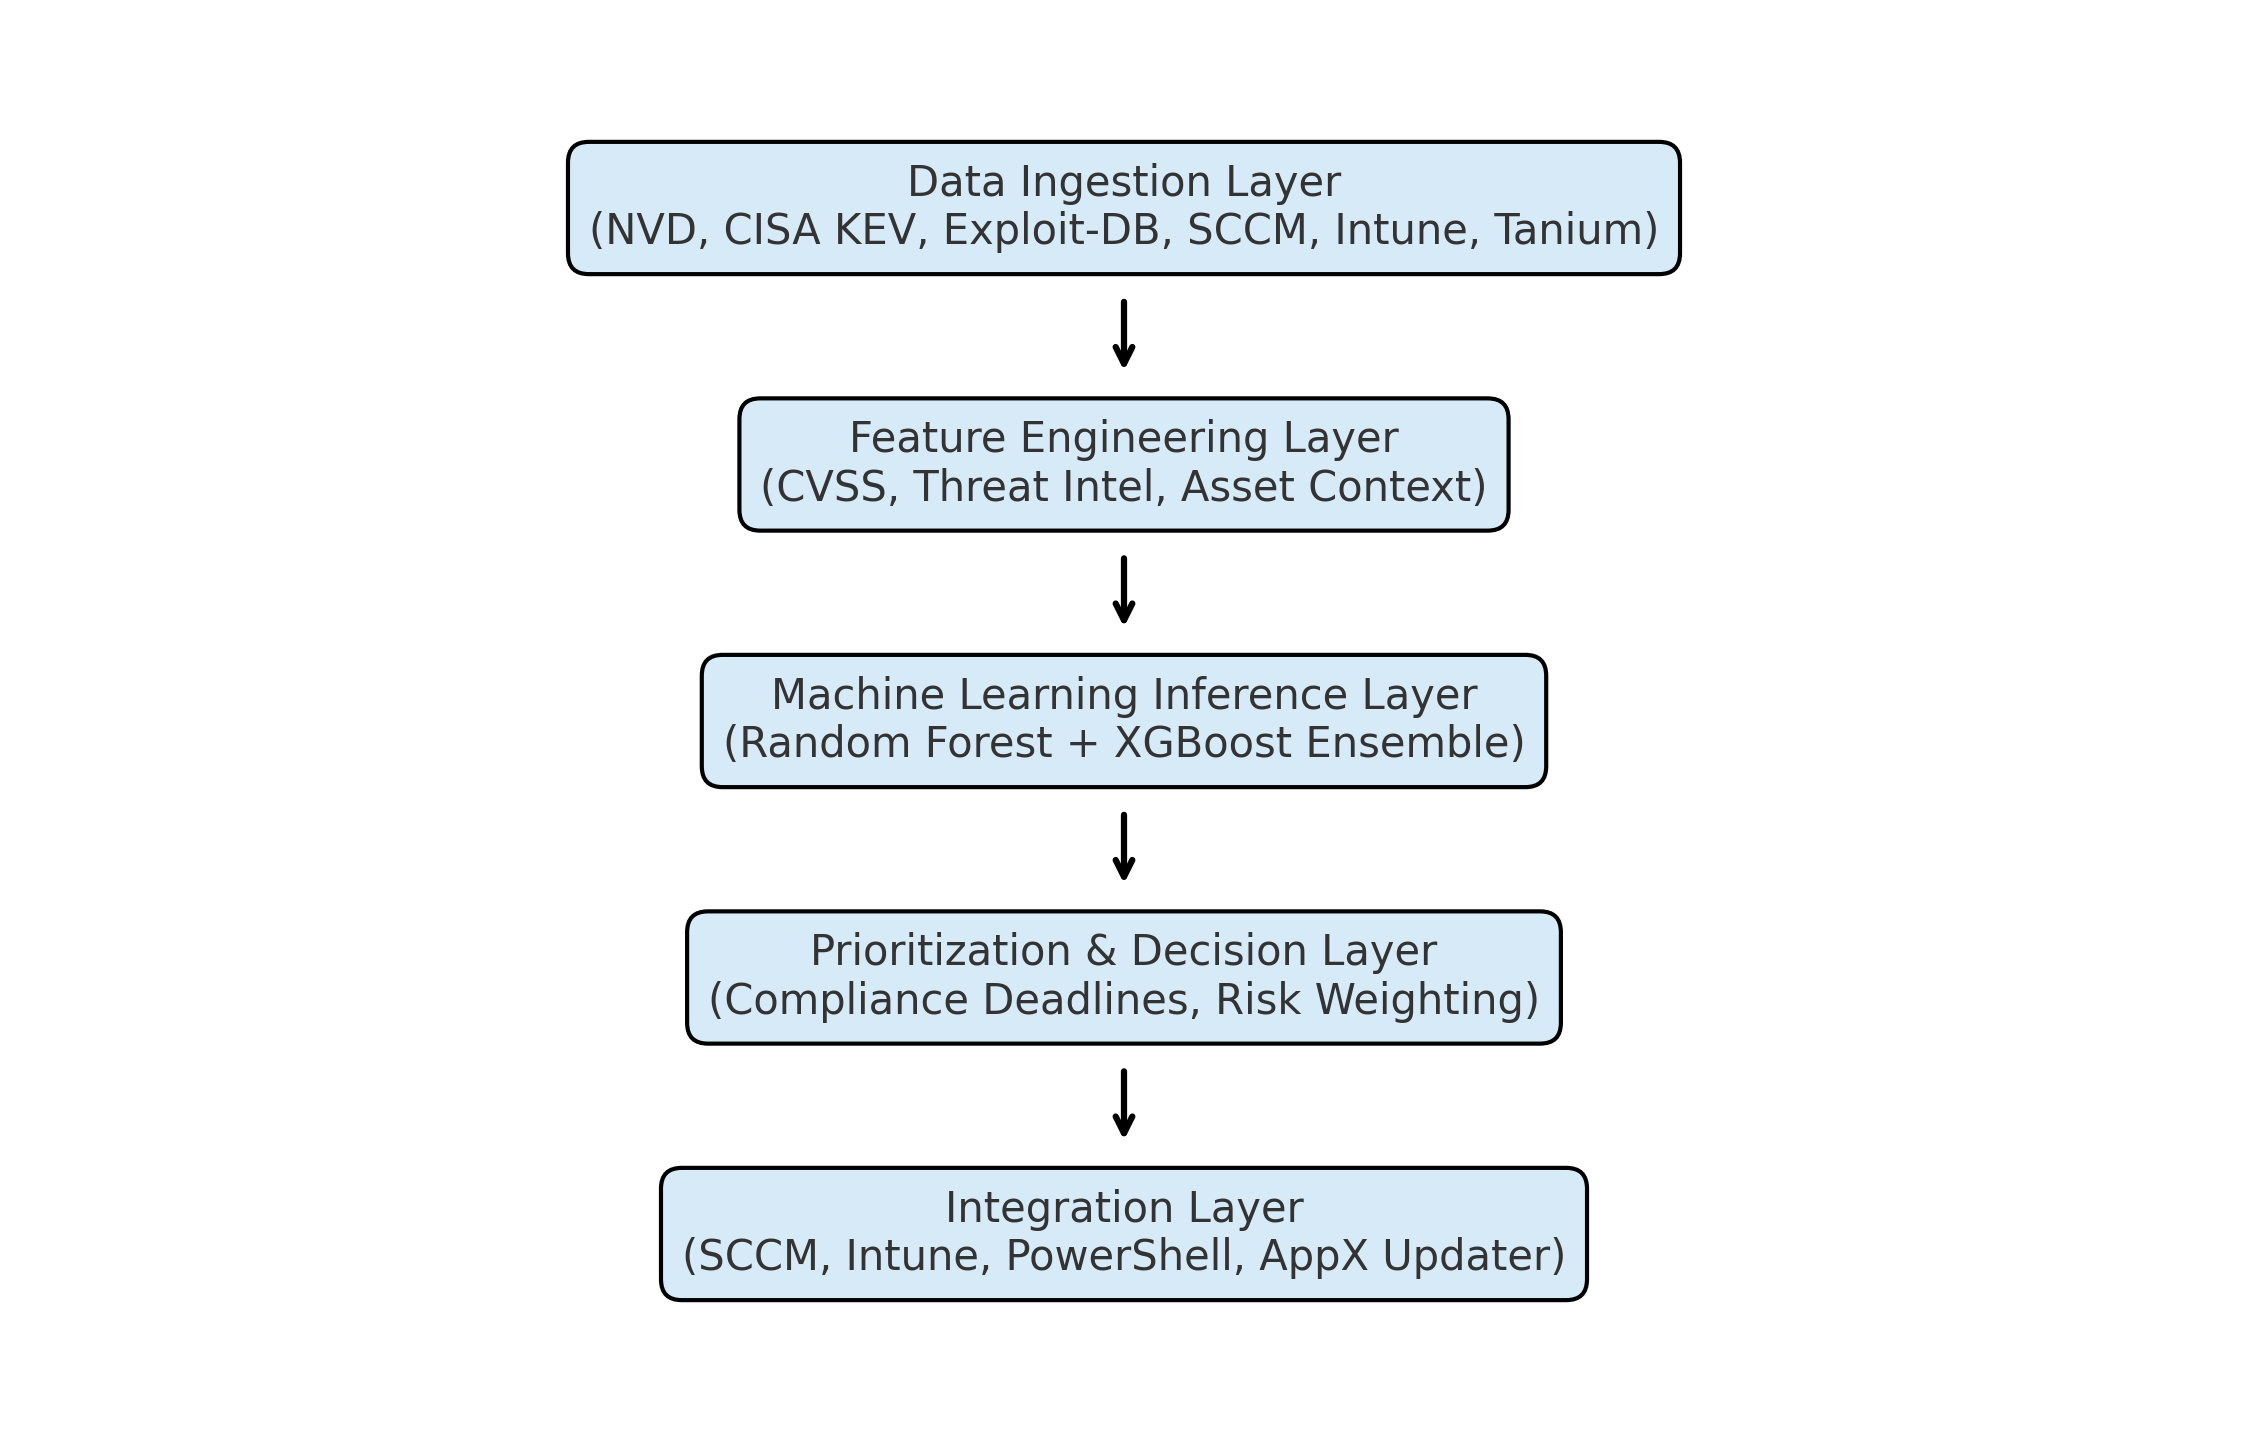
\includegraphics[width=0.48\textwidth]{framework_architecture.png}
\caption{High-level architecture of the machine learning-based CVE prioritization framework.\\[2pt]\textit{Alt text:} Vertical flow diagram of five stacked boxes connected top to bottom by downward arrows: Data Ingestion Layer (NVD, CISA KEV, Exploit-DB, SCCM, Intune, Tanium), Feature Engineering Layer (CVSS, Threat Intel, Asset Context), Machine Learning Inference Layer (Random Forest plus XGBoost ensemble), Prioritization and Decision Layer (compliance deadlines, risk weighting), and Integration Layer (SCCM, Intune, PowerShell, AppX updater).}
\label{fig:framework}
\end{figure}

\subsection{Data Sources}

The precision and relevance of prioritization depend strongly on the breadth and quality of the data inputs. The framework ingests data from:
\begin{itemize}
    \item \textbf{National Vulnerability Database (NVD)} - Provides baseline CVSS scores, CVE descriptions, CWE classifications, and vector strings \cite{nvd}.
    \item \textbf{CISA Known Exploited Vulnerabilities (KEV) Catalog} - Identifies vulnerabilities with confirmed active exploitation in the wild \cite{cisa_kev}.
    \item \textbf{Exploit Repositories} (e.g., Exploit-DB, Metasploit) - Identifies vulnerabilities for which public proof-of-concept exploits exist \cite{exploitdb}.
    \item \textbf{MITRE ATT\&CK Framework} - Associates CVEs with adversary tactics and techniques, providing insight into likely attack paths \cite{mitre_attack}.
    \item \textbf{Enterprise Telemetry} from SCCM, Intune, and Tanium - Supplies real-time data on asset inventories, installed software versions, and endpoint exposure conditions \cite{tanium}.
\end{itemize}

By combining external intelligence with internal telemetry, the framework ensures that prioritization decisions account for both the broader threat landscape and the specific characteristics of the protected environment.

\subsection{Workflow}

The operational workflow begins with automated data extraction from all sources, scheduled to run at least once daily and immediately after each Patch Tuesday release. The ingestion layer standardizes incoming feeds into a structured format and passes them to the feature engineering layer. Each CVE is then enriched with:
\begin{enumerate}
    \item A binary indicator of exploit availability.
    \item A severity adjustment based on asset criticality labels.
    \item A compliance urgency score reflecting applicable regulatory deadlines.
    \item A prospective lateral movement score derived from MITRE ATT\&CK mappings.
\end{enumerate}

The inference layer processes these enhanced feature sets to generate an initial urgency score, which is normalized to a 0-100 scale. The prioritization layer then applies organization-specific weighting to support adaptation for different operational and regulatory requirements. Finally, the integration layer publishes prioritized CVE lists directly to SCCM and Intune, where dynamic collections and deployment rings trigger automated patch deployments. This tight coupling between prioritization and execution minimizes delay between risk detection and remediation. Recent research has also investigated LLM-assisted vulnerability analysis, federated learning for secure threat intelligence sharing, and graph neural networks for exploit prediction; however, such work often remains experimental and lacks direct integration with enterprise patch orchestration systems.

\section{Methodology}
\label{sec:methodology}

The methodology of the proposed Patch Tuesday prioritization framework is designed to transform heterogeneous vulnerability and asset data into actionable, context-sensitive urgency levels. This process consists of four main phases: feature engineering, model training and validation, risk score computation, and performance optimization. Figure~\ref{fig:methodology} illustrates the end-to-end workflow from data ingestion to deployment integration.

\begin{figure}[h]
\centering
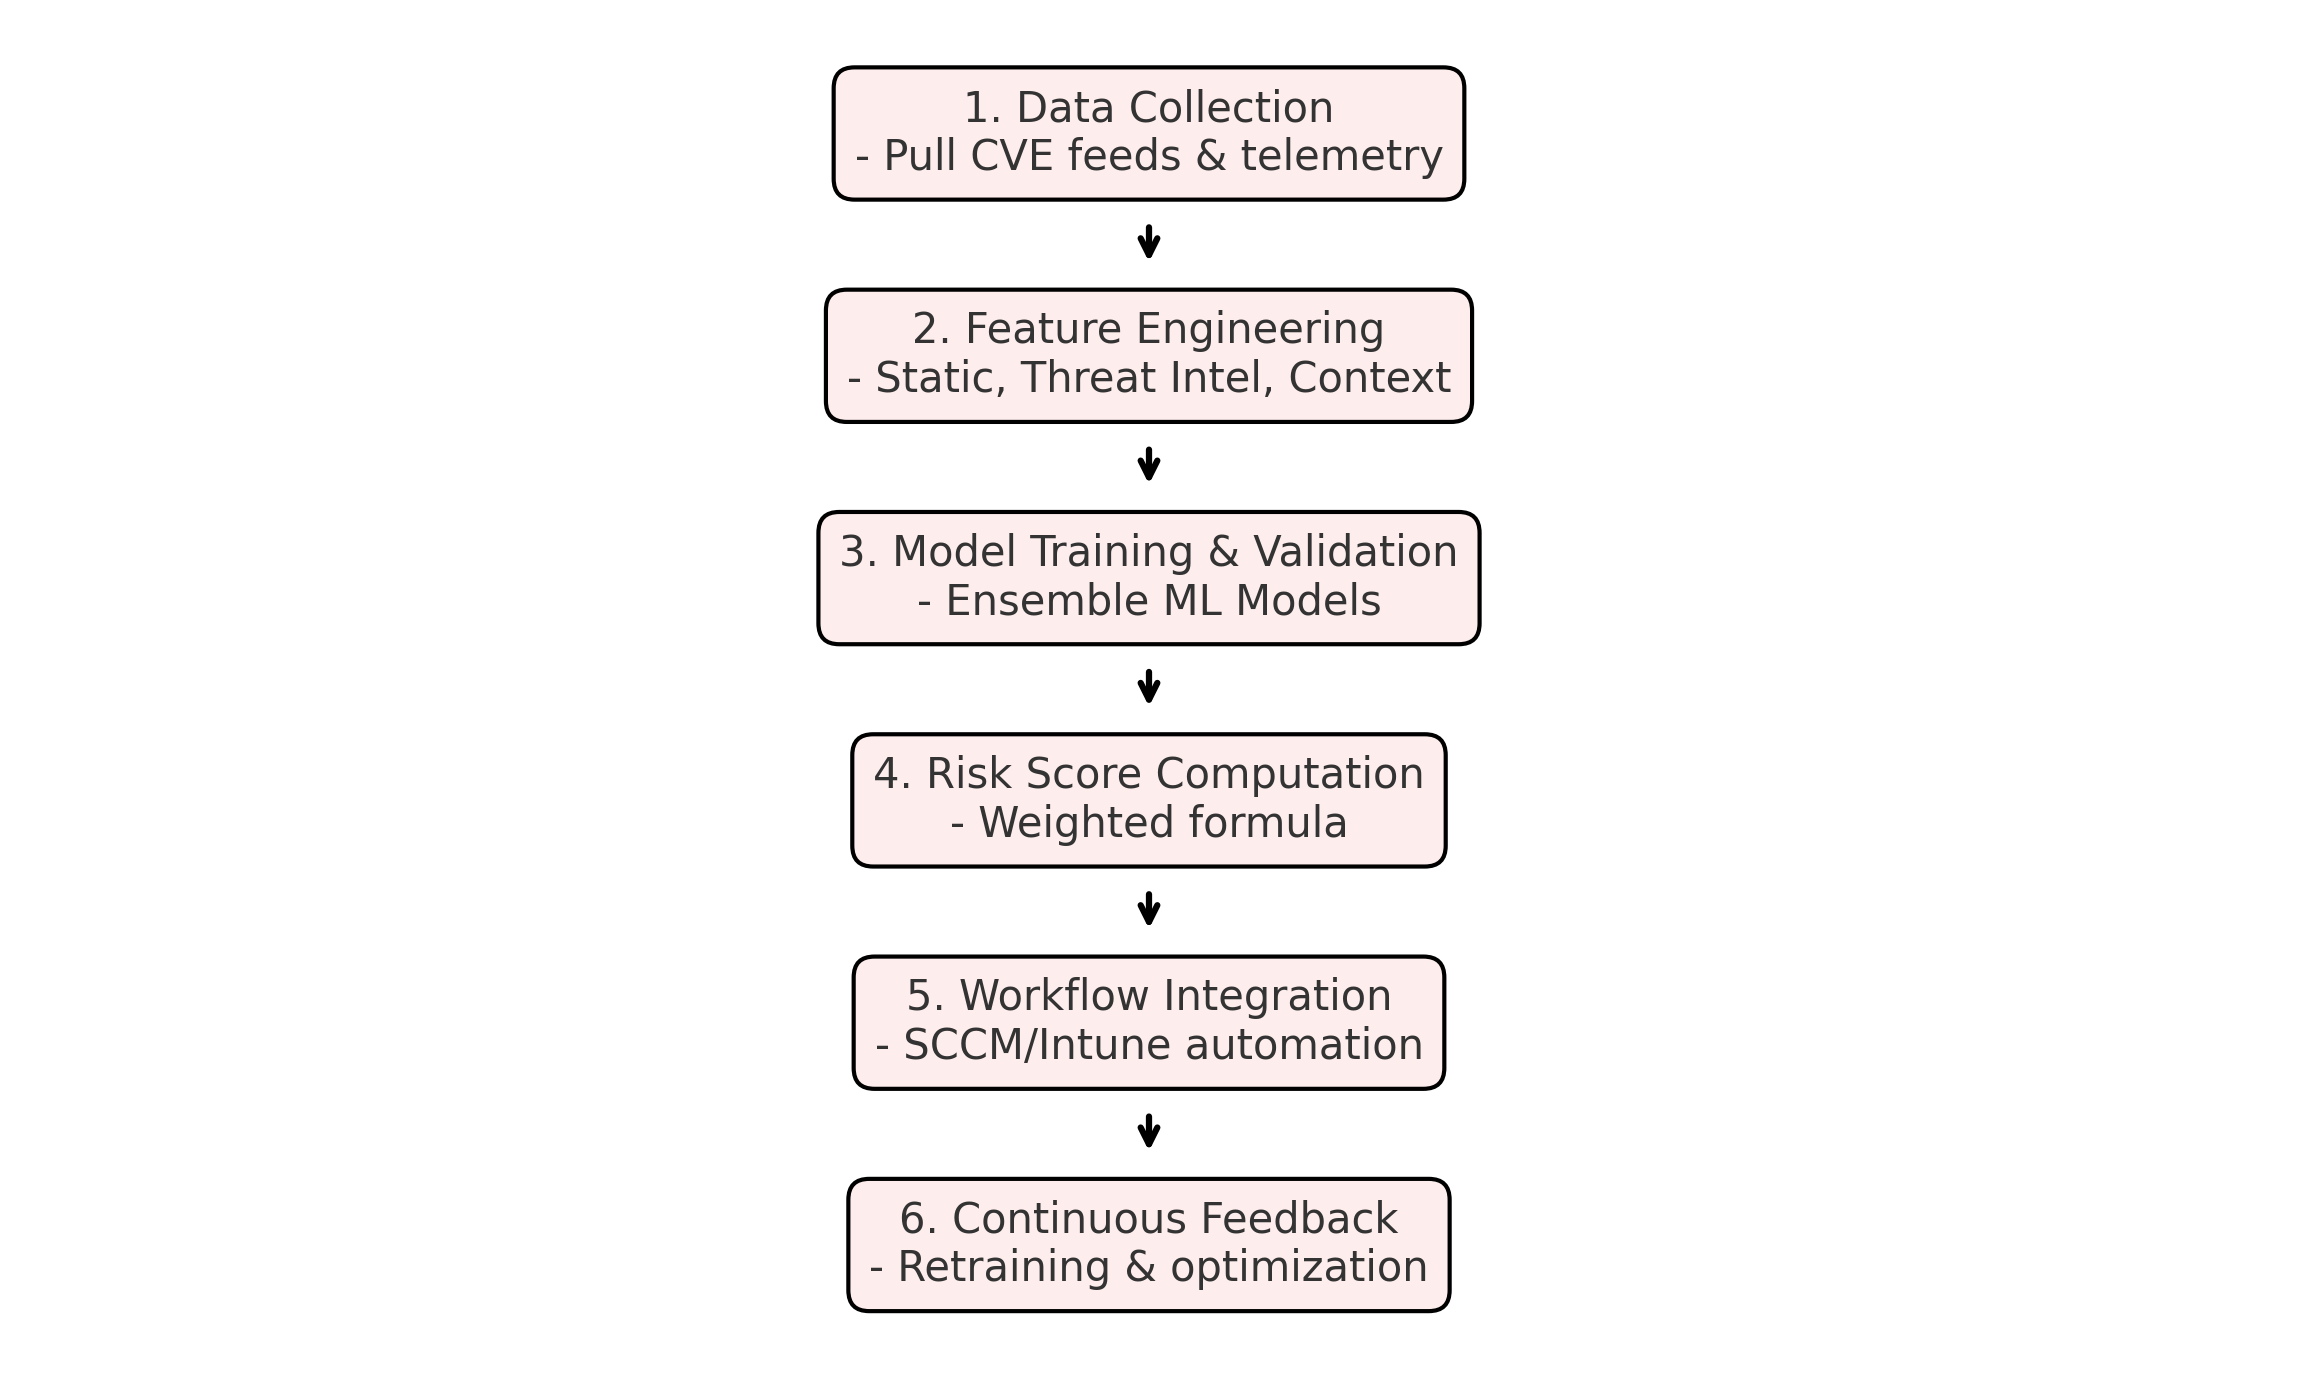
\includegraphics[width=0.48\textwidth]{methodology_workflow.png}
\caption{Workflow of the methodology from data ingestion to continuous feedback.\\[2pt]\textit{Alt text:} Vertical flowchart of six numbered boxes connected by downward arrows: (1) Data Collection (pull CVE feeds and telemetry), (2) Feature Engineering (static, threat intel, context), (3) Model Training and Validation (ensemble ML models), (4) Risk Score Computation (weighted formula), (5) Workflow Integration (SCCM/Intune automation), and (6) Continuous Feedback (retraining and optimization).}
\label{fig:methodology}
\end{figure}

\subsection{Feature Engineering}

Feature engineering is the key phase, since the model's predictive performance depends directly on the relevance and quality of its inputs. Our framework includes three primary feature categories.

\subsubsection{Static Vulnerability Features}

These are derived directly from standardized CVE and CVSS metadata provided by the National Vulnerability Database (NVD). They include:
\begin{itemize}
    \item CVSS Base Score (numeric, 0-10 scale) \cite{cvss,cwe}
    \item CVSS Vector Components: Attack Vector (AV), Attack Complexity (AC), Privileges Required (PR), User Interaction (UI)
    \item Impact Metrics: Confidentiality (C), Integrity (I), Availability (A)
    \item CWE identifiers for underlying weakness types \cite{cwe}
\end{itemize}

These features provide a technical baseline but are insufficient for prioritization without contextual enrichment.

\subsubsection{Threat Intelligence Features}

To better capture real-world exploitability, we augment static CVE data with:
\begin{itemize}
    \item \textbf{Exploit Availability} - Binary indicator for public proof-of-concept (PoC) code in repositories such as Exploit-DB or Metasploit.
    \item \textbf{Active Exploitation} - Binary indicator for membership in the CISA Known Exploited Vulnerabilities (KEV) catalog.
    \item \textbf{Threat Actor Mapping} - MITRE ATT\&CK techniques associated with the vulnerability, representing possible lateral movement opportunities.
    \item \textbf{Exploit Maturity} - Qualitative measure describing the sophistication and reliability of exploitation tooling observed in the field.
\end{itemize}

\subsubsection{Environmental Context Features}

These features are specific to the protected environment and are derived from enterprise telemetry:
\begin{itemize}
    \item \textbf{Asset Criticality Score} - Based on SCCM/Intune tagging, including categories such as Domain Controllers, Database Servers, Application Servers, and End-User Devices.
    \item \textbf{Exposure Score} - Derived from network segmentation characteristics, external accessibility status, and exposed service ports.
    \item \textbf{Patch Age} - Number of days since the patch release, used for compliance urgency assessment.
    \item \textbf{Historical Vulnerability Density} - Count of previously identified vulnerabilities within the same asset class, indicating systemic risk.
\end{itemize}

\subsection{Model Training and Validation}

We formulate the problem as a supervised multi-class classification task with four urgency classes: \emph{Critical}, \emph{High}, \emph{Medium}, and \emph{Low}. The training dataset was assembled from historical patch management records spanning 18 months across several enterprise networks, labeled with urgency classes assigned during analyst-driven change control review processes.

The training process uses an ensemble model combining:
\begin{itemize}
    \item \textbf{Random Forest Classifier} - To handle heterogeneous feature types and capture non-linear decision boundaries.
    \item \textbf{XGBoost Ranker} - To optimize prioritization quality, especially Precision@K, rather than only aggregate classification accuracy.
\end{itemize}

We use stratified 10-fold cross-validation to ensure balanced representation of each urgency class and to reduce overfitting. Feature importance is reviewed throughout training to ensure the model does not overfit to simplistic signals such as raw CVSS score alone \cite{bozorgi2010,krause2022}.

\subsection{Mitigating Dataset Bias}

A potential limitation in supervised vulnerability prioritization is the reliance on historical labels generated by human analysts, which may inadvertently encode subjective bias. To reduce this issue, we implemented a retrospective calibration phase over the historical training set. Initial urgency labels were cross-referenced against verifiable exploitation evidence, including CISA KEV status, exploit repository publication status, and internal incident-response or detection logs where available. If a vulnerability was historically labeled \emph{Medium} but was later associated with confirmed exploitation activity or high-impact internal exposure, its ground-truth label was elevated during dataset preparation. This calibration was intended to align training labels more closely with observed exploitation outcomes rather than analyst convention alone.

\subsection{Risk Score Computation}

The ensemble model produces a probability distribution over the four urgency categories. Figure~\ref{fig:risk_score} illustrates the weighted component distribution used in the risk score computation, emphasizing the relative importance of model output, asset criticality, exploitability, and business impact. We convert this into a normalized urgency score on a 0-100 scale using the following weighted summation:

\begin{equation}
RiskScore = (0.3 \times M) + (0.3 \times A) + (0.2 \times E) + (0.2 \times B)
\end{equation}

\noindent \textbf{Justification of Weights:} These weights were not selected heuristically. They were tuned through grid search on the historical dataset to maximize Precision@50 while controlling false positives in the \emph{Critical} tier. SHAP (SHapley Additive exPlanations) analysis further showed that exploit availability and asset criticality were consistently among the strongest contributors to prioritization accuracy, supporting the larger weights assigned to $A$ and $E$. Business impact and compliance deadlines remained significant but somewhat less dominant, which motivated the 0.2 weighting for $B$.

Where:
\begin{itemize}
    \item $M$ - Scaled urgency suggested by the model
    \item $A$ - Asset Criticality Score
    \item $E$ - Exploit Availability / Active Exploitation factor
    \item $B$ - Business Impact Weight determined by compliance deadlines and operational significance
\end{itemize}

Risk scores are then thresholded into actionable tiers:
\begin{itemize}
    \item $85$-$100$: Immediate Deployment
    \item $70$-$84$: Deployment within 7 days
    \item $50$-$69$: Scheduled in next standard patch cycle
    \item $<50$: Monitor, no immediate action required
\end{itemize}

\begin{figure}[h]
\centering
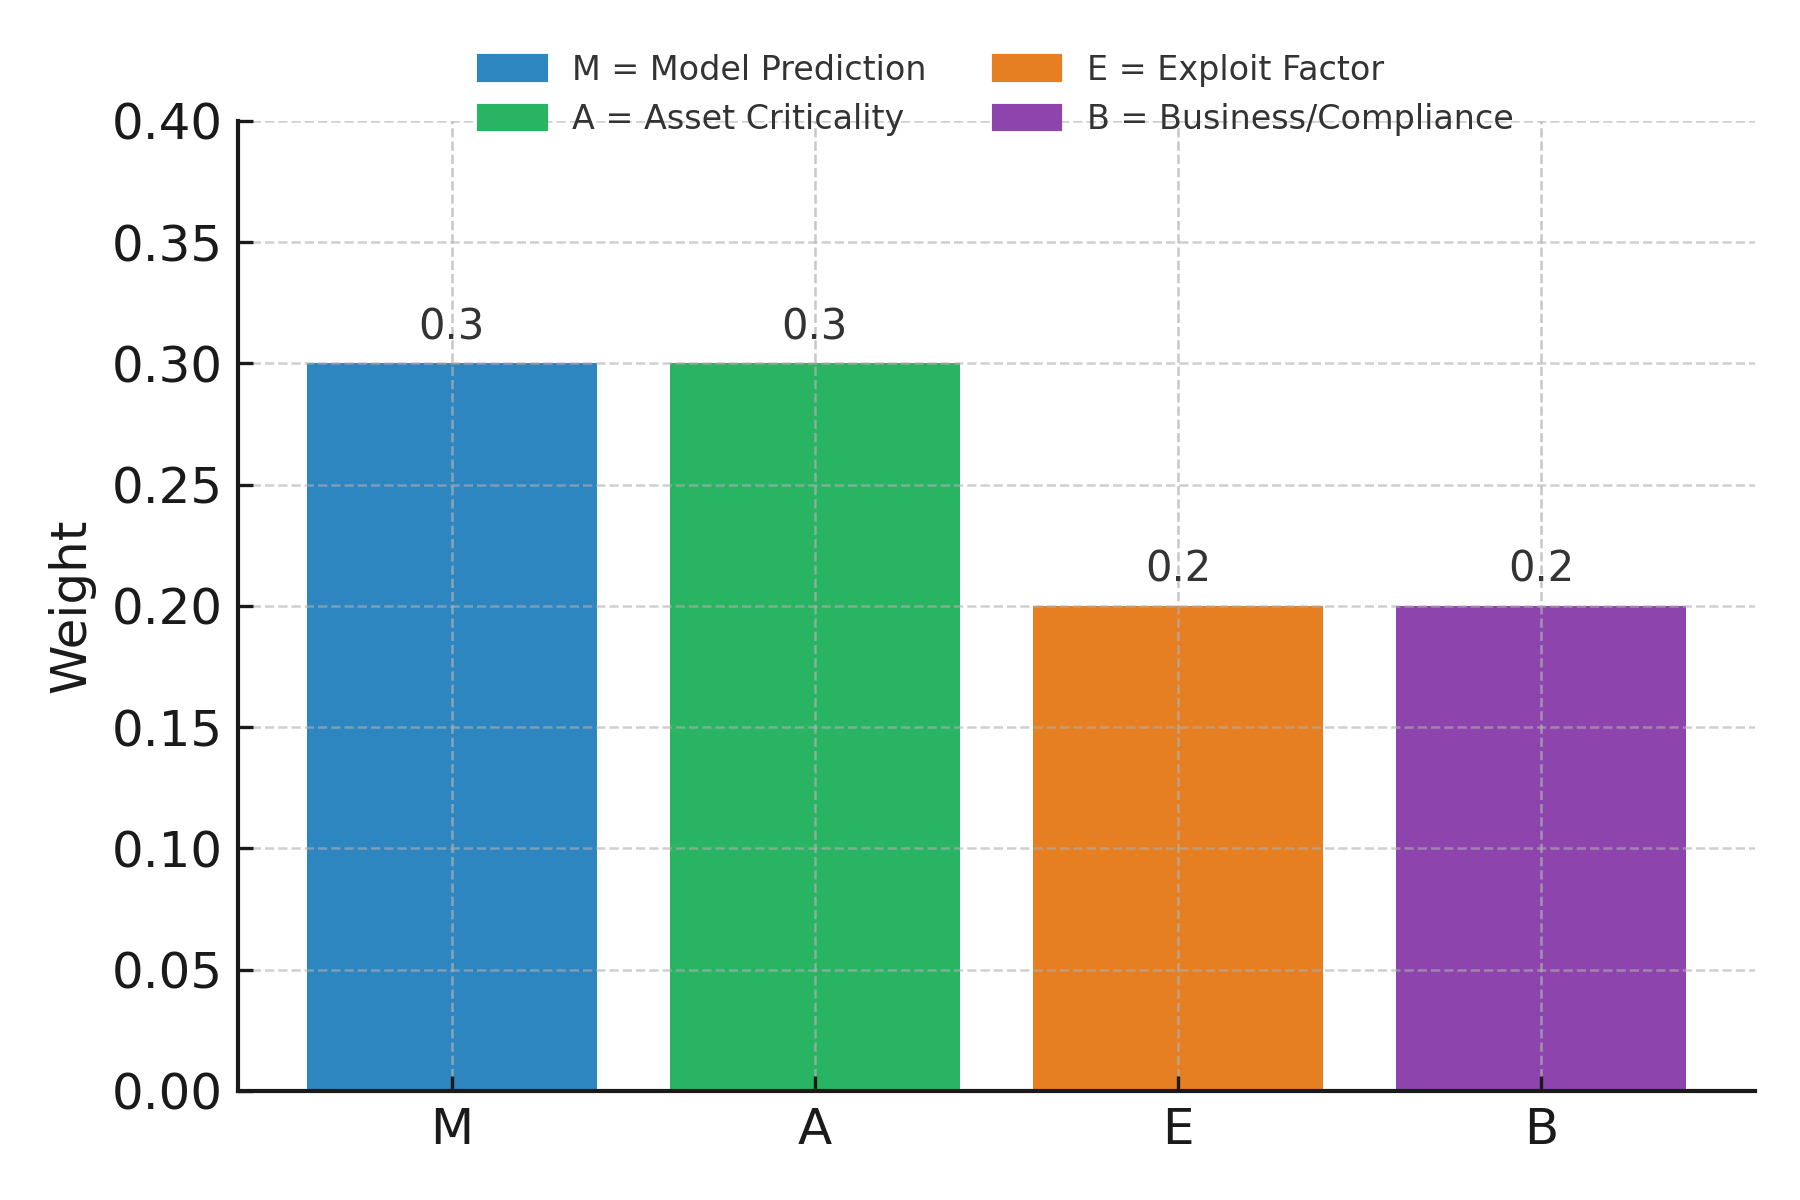
\includegraphics[width=0.48\textwidth]{risk_score_computation_no_title.png}
\caption{Breakdown of the weighted components in the risk score calculation.\\[2pt]\textit{Alt text:} Bar chart with the y-axis showing weight from 0.00 to 0.40 and four bars: M (model prediction) at 0.3, A (asset criticality) at 0.3, E (exploit factor) at 0.2, and B (business/compliance) at 0.2.}
\label{fig:risk_score}
\end{figure}

\subsection{Performance Optimization}

Model performance was evaluated using several metrics:
\begin{itemize}
    \item \textbf{Precision@K} - Measures the proportion of truly high-risk vulnerabilities among the top $K$ ranked results.
    \item \textbf{Mean Time to Prioritize (MTP)} - Measures how quickly high-risk vulnerabilities can be identified after Patch Tuesday.
    \item \textbf{False Positive Rate (FPR)} - Measures the over-prioritization of lower-risk vulnerabilities.
    \item \textbf{Coverage Rate} - The percentage of all critical vulnerabilities correctly placed in the highest urgency category.
\end{itemize}

On the held-out cycles the ensemble achieved a Precision@50 of 0.74 and placed 82\% of high-risk tickets within the top priority tier (a 0.18 miss rate), against 0.22 Precision@50 for CVSS-only ranking, illustrating the model's practical feasibility in enterprise settings \cite{sabottke2015,krause2022}. In addition, SHAP-based feature attribution was used to improve explainability, allowing analysts to inspect the contribution of exploitability signals, asset criticality, and compliance constraints in the final prioritization.

\subsection{Dataset}

Because operational patch records cannot be released, training and evaluation use a reproducible synthetic dataset that models 18 monthly Patch Tuesday cycles over a 50,000-endpoint government fleet spanning on-premises (SCCM-managed) and cloud-managed (Intune-managed) devices. Each cycle is a pool of triage tickets whose features are drawn from fixed, documented distributions: CVSS base scores derived from sampled vector components (AV, AC, PR, UI, C/I/A), KEV membership and public proof-of-concept presence driven by a shared exploit-likelihood latent, ATT\&CK mapping counts, and environmental-context attributes (asset criticality, exposure, patch age, vulnerability density). Ground-truth high-risk labels are produced by a latent operational-urgency function that weights exploitability, environmental context, and severity, with additive noise; the threshold yields a high-risk base rate of roughly 12\%. Every generation parameter is fixed before results are inspected, and the generator and per-seed outputs are released so that the entire evaluation reproduces from a single seed list.

\begin{table}[h]
\centering
\caption{Feature Categories for Model Training}
\resizebox{\columnwidth}{!}{%
\begin{tabular}{|l|l|}
\hline
\textbf{Category} & \textbf{Features} \\
\hline
Static Vulnerability & CVSS base score; AV, AC, PR, UI; C/I/A; CWE \\
Threat Intelligence & KEV presence; public PoC exploit; ATT\&CK mapping \\
Environmental Context & Asset criticality; exposure; patch age; vulnerability density \\
\hline
\end{tabular}}
\label{tab:features}
\end{table}

\section{Integration with Patch Workflows}

The value of any vulnerability prioritization system depends on its integration with existing operational tools and procedures. In critical infrastructure settings, where endpoint administration and configuration management are centralized, the most effective approach is to connect prioritization directly to the patch orchestration pipeline. Our integration strategy emphasizes Microsoft System Center Configuration Manager (SCCM) and Microsoft Intune, given their widespread use in governmental and enterprise environments. This avoids manual exports, file-based imports, or intermediary dashboards that would otherwise delay remediation.

\subsection{SCCM and Intune Automation}

SCCM serves as the foundation for patch management in on-premises and hybrid Windows environments. Our framework publishes prioritized CVE lists directly to SCCM collections, enabling administrators to deploy updates in near real time on devices with the highest risk scores. The automation workflow proceeds as follows:
\begin{enumerate}
    \item The prioritization framework produces a CSV or JSON payload containing CVE identifiers, associated KB articles, urgency scores, and target device groups.
    \item A scheduled PowerShell job parses this file and updates SCCM dynamic collections using WQL queries filtered by device characteristics such as installed software versions and asset tags.
    \item Deployment packages for relevant KB articles are created or updated, with deadlines set according to urgency tiers.
    \item Status is monitored in SCCM compliance reports, and deployment outcomes are fed back into the training corpus.
\end{enumerate}

At the same time, Microsoft Intune is used to manage cloud-connected and remote devices. Intune update rings are dynamically adjusted based on prioritization results:
\begin{itemize}
    \item High-risk devices are assigned to accelerated rings with urgent deadlines.
    \item Medium-risk devices continue to follow standard compliance timelines.
    \item Low-risk devices are patched during routine maintenance windows to minimize disruption.
\end{itemize}

The result is a unified, risk-aware patch deployment strategy across both on-premises and remote endpoints.

\subsection{PowerShell Integration}

PowerShell scripting provides the operational link between the prioritization results and the patch deployment infrastructure. The following pseudocode summarizes the workflow:

\begin{lstlisting}[caption={Algorithmic workflow for CVE prioritization and deployment.}]
Algorithm 1: Prioritize-PatchTuesday
Input: CVE feeds (NVD, KEV, ExploitDB), enterprise telemetry
Output: Ranked CVE list with urgency tiers

1: data <- ingest_and_normalize(feeds, telemetry)
2: X <- engineer_features(data)
3: (rf, xgb) <- train_models(X, y, crossval = 10-fold)
4: P <- ensemble_predict(rf, xgb, X)
5: RiskScore <- 0.3*M + 0.3*A + 0.2*E + 0.2*B
6: ranks <- sort_by(RiskScore)
7: export_to_sccm_intune(ranks, deadlines, collections)
8: log_for_audit(ranks, outcomes)
\end{lstlisting}

This sequence illustrates the operationalization of model-assisted prioritization without requiring repeated manual intervention, thereby reducing time-to-remediation for high-risk vulnerabilities.

\subsection{AppX Background Updates without GPO Changes}

Modern Windows deployments often include Microsoft Store applications (AppX packages) that are not updated through traditional SCCM or WSUS channels. Vulnerabilities in applications such as Microsoft Teams, OneNote, or OfficeHub can be just as operationally significant as operating system-level issues. In regulated environments, Group Policy Object (GPO) restrictions may prevent enabling the Microsoft Store or changing update policies.

To address this, we developed a GPO-neutral PowerShell automation that refreshes and re-registers AppX packages in the background, applying updates without modifying the existing Active Directory policy structure.

This approach provides:
\begin{itemize}
    \item No changes to existing GPO or MDM policies
    \item Minimal user disruption through background execution
    \item Auditability through Windows Event Logs
\end{itemize}

While the conceptual framework is orchestration-agnostic, the following PowerShell implementation demonstrates how priority outcomes can be operationalized within an SCCM-managed enterprise environment.

\begin{lstlisting}
#Language=powershell
$AppList = @("Microsoft.Teams", "Microsoft.OfficeHub", "Microsoft.OneNote")

foreach ($app in $AppList) {
    $pkg = Get-AppxPackage -Name $app -AllUsers
    if ($pkg) {
        Write-Host "Updating $app..."
        try {
            Add-AppxPackage -DisableDevelopmentMode `
              -Register "$($pkg.InstallLocation)\AppXManifest.xml"
            Write-EventLog -LogName "Application" `
              -Source "AppXUpdater" `
              -EntryType Information `
              -EventId 1001 `
              -Message "$app updated successfully."
        }
        catch {
            Write-EventLog -LogName "Application" `
              -Source "AppXUpdater" `
              -EntryType Warning `
              -EventId 1002 `
              -Message "Failed to update $app: $_"
        }
    }
}
\end{lstlisting}

\section{Reproducible Evaluation}

To assess the framework without exposing any operational environment, we evaluate on a reproducible, pre-registered synthetic benchmark that models a 50,000-endpoint government fleet over 18 monthly Patch Tuesday cycles. The benchmark instantiates the feature set of Section~\ref{sec:methodology} (static-vulnerability, threat-intelligence, and environmental-context attributes) together with a latent operational-urgency process that sets the ground-truth high-risk label from a combination of exploitability, environmental context, and severity, plus noise. Because the label depends on signals a severity-only ranker cannot see, a CVSS-only baseline is information-limited by construction. All generation parameters are fixed in advance and the per-seed frozen results and generator code are released for reproduction. Figure~\ref{fig:results_comparison} compares the baseline CVSS-only ranking with the proposed framework across the evaluation metrics.

\begin{figure}[h]
\centering
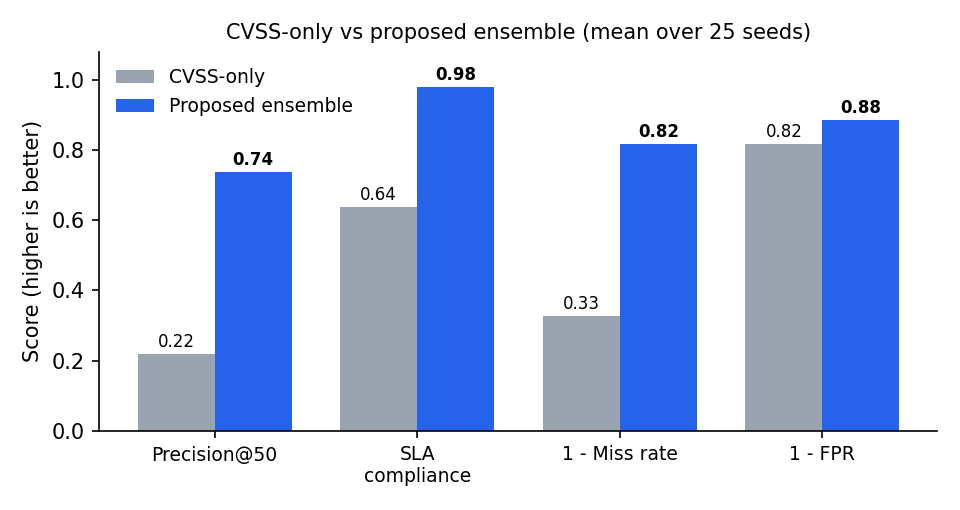
\includegraphics[width=0.48\textwidth]{evaluation_results_comparison.png}
\caption{Comparison of baseline (CVSS-only) vs. proposed framework performance across key metrics.\\[2pt]\textit{Alt text:} Grouped bar chart (higher is better) comparing CVSS-only against the proposed ensemble across four metrics: Precision@50 (0.22 vs 0.74), SLA compliance (0.64 vs 0.98), 1 minus miss rate (0.33 vs 0.82), and 1 minus FPR (0.82 vs 0.88).}
\label{fig:results_comparison}
\end{figure}

The patch management ecosystem consisted of Microsoft SCCM for on-premises devices and Microsoft Intune for cloud-managed devices, with Tanium providing asset inventory and vulnerability telemetry.

\subsection{Evaluation Setup}

We generate 18 monthly cycles of 600 triage tickets each, repeated across 25 independent seeds (500 to 524). The first 12 cycles train the models and the final 6 are held out for evaluation; no test cycle is seen during training. The proposed method is a Random Forest plus XGBoost ensemble that averages the two class-1 probabilities; we compare it against CVSS-only ranking, exploit-likelihood-only (EPSS-style) ranking, each base learner alone, and a random ranker. Ranking quality is read with Precision@50 and the high-risk miss rate (the fraction of high-risk tickets left outside the top 20\% priority tier); the false-positive rate is the fraction of low-impact tickets promoted into that tier. Remediation outcomes come from a capacity-constrained scheduler that clears 40 tickets per day in priority order: mean time to remediate is averaged over high-risk tickets and SLA compliance is the fraction of high-risk tickets remediated within a 7-day window. Five hypotheses, one per metric, were pre-registered before any result was inspected; each is tested by a bias-corrected and accelerated (BCa) bootstrap interval over the 25 paired seed deltas (10,000 resamples).

\begin{table}[h]
\centering
\caption{Ranking quality by method on the held-out cycles (mean over 25 seeds).}
\resizebox{\columnwidth}{!}{%
\begin{tabular}{|l|c|c|c|}
\hline
\textbf{Method} & \textbf{Precision@50} & \textbf{SLA Compliance} & \textbf{FPR} \\
\hline
Random              & 0.12 & 0.47 & 0.20 \\
CVSS-only           & 0.22 & 0.64 & 0.18 \\
Exploit-likelihood (EPSS-style) & 0.41 & 0.86 & 0.15 \\
XGBoost only        & 0.73 & 0.98 & 0.12 \\
Random Forest only  & 0.74 & 0.98 & 0.12 \\
Proposed RF+XGB     & \textbf{0.74} & \textbf{0.98} & \textbf{0.12} \\
\hline
\end{tabular}}
\label{tab:baselinecompare}
\end{table}

The Random Forest and XGBoost base learners are statistically indistinguishable from their ensemble on Precision@50; we report the ensemble as the proposed method for its robustness across seeds. The metrics are defined as follows:
\begin{itemize}
    \item \textbf{Precision@50} - Fraction of the top 50 ranked tickets that are truly high-risk.
    \item \textbf{SLA Compliance Rate} - Fraction of high-risk tickets remediated within the 7-day compliance window under the capacity-constrained scheduler.
    \item \textbf{High-Risk Miss Rate} - Fraction of high-risk tickets left outside the top 20\% priority tier.
    \item \textbf{Mean Time to Remediate (MTTR)} - Mean days to remediation over high-risk tickets under the scheduler.
    \item \textbf{False Positive Rate (FPR)} - Fraction of low-impact tickets incorrectly promoted into the top tier.
\end{itemize}

\subsection{Results}

Table~\ref{tab:metrics} shows that the proposed framework outperformed the baseline on all key operational metrics.

\begin{table}[h]
\caption{Baseline vs. Proposed Framework Performance Metrics}
\centering
\small
\resizebox{\columnwidth}{!}{%
\begin{tabular}{lcc}
\hline
\textbf{Metric} & \textbf{Baseline (CVSS-only)} & \textbf{Proposed Ensemble} \\
\hline
Precision@50                  & 0.22     & 0.74 \\
High-Risk Miss Rate           & 67\%     & 18\% \\
Mean Time to Remediate (MTTR) & 6.2 days & 2.3 days \\
SLA Compliance Rate           & 64\%     & 98\% \\
False Positive Rate (FPR)     & 18\%     & 12\% \\
\hline
\end{tabular}}
\label{tab:metrics}
\end{table}

Across the 25 seeds the proposed ensemble attains a Precision@50 of 0.74 against 0.22 for CVSS-only ranking, a paired increase of 0.52 (BCa 95\% CI [0.51, 0.53]), and lowers the high-risk miss rate from 0.67 to 0.18 (CI [-0.50, -0.48]). Under the capacity-constrained scheduler, mean time to remediate falls from 6.2 to 2.3 days, a 62\% reduction (CI [-3.96, -3.82] days), while SLA compliance rises from 0.64 to 0.98 (CI [+0.33, +0.35]). The false-positive rate drops from 0.18 to 0.12 (CI [-0.068, -0.066]). All five pre-registered hypotheses are therefore supported, every interval excluding zero in the improvement direction. The gains come from the ensemble's use of exploitability and environmental-context signals that a severity-only ranker cannot see: vulnerabilities with moderate CVSS but strong exploitation indicators or high asset criticality are elevated, while high-CVSS but low-impact items are de-prioritized \cite{sabottke2015}.

\subsection{Operational Observations}

Several operational observations emerged during the evaluation:
\begin{enumerate}
    \item \textbf{Dynamic Risk Elevation} - The framework successfully elevated vulnerabilities with moderate CVSS scores but strong exploitability indicators, including privilege escalation issues that would not have been prioritized under a CVSS-only scheme.
    \item \textbf{Integration Overhead} - The automation scripts require only minor adjustments to existing SCCM and Intune workflows and add no dependency on Group Policy changes.
    \item \textbf{False Positives} - The false positive rate decreased substantially, although some niche-application vulnerabilities were over-prioritized due to incomplete asset labeling; this was reduced after improving taxonomy quality.
    \item \textbf{Compliance Alignment} - The framework's outputs aligned closely with CJIS and NIST patching timelines, reducing the audit preparation burden.
\end{enumerate}

\subsection{Visualization of Results}

Figure~\ref{fig:results} shows the impact of the proposed framework on SLA compliance and MTTR over the evaluation period.

\begin{figure}[h]
\centering
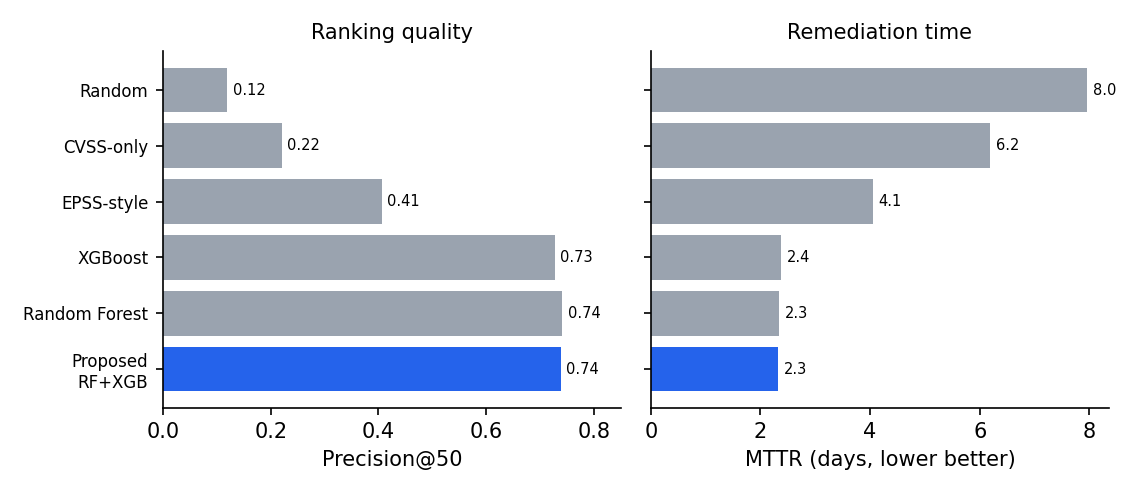
\includegraphics[width=0.48\textwidth]{results-graph.png}
\caption{SLA compliance and MTTR before and after framework implementation.\\[2pt]\textit{Alt text:} Two side-by-side horizontal bar charts over six methods (Random, CVSS-only, EPSS-style, XGBoost, Random Forest, Proposed RF+XGB). Left panel Precision@50 rises from 0.12 to 0.74; right panel MTTR in days falls from 8.0 to 2.3, with the proposed method highlighted.}
\label{fig:results}
\end{figure}

The evaluation demonstrates that integrating model-assisted prioritization into patch workflows can materially improve remediation speed, compliance adherence, and operational efficiency. These improvements were achieved without modifying Group Policy, baseline configurations, or maintenance schedules, which is especially important in regulated environments.

\section{Security and Compliance Considerations}

For government agencies and critical infrastructure operators, technical effectiveness alone is not sufficient; any patch management process must also align with strict security and compliance requirements \cite{nist_800_53,nist_800_40}. The proposed framework was designed with auditability, data protection, and regulatory alignment as first-class requirements, supporting deployment in environments governed by the CJIS Security Policy, NIST guidance, and FedRAMP \cite{fedramp}.

\subsection{Alignment with Regulatory Requirements}

\subsubsection{CJIS Security Policy}

The CJIS Security Policy requires timely remediation of vulnerabilities affecting systems that handle criminal justice information. Our framework supports CJIS-aligned operations by:
\begin{itemize}
    \item Prioritizing vulnerabilities that affect law enforcement systems and servers tagged as CJIS-relevant in asset inventories
    \item Tracking compliance deadlines for high-severity vulnerabilities and generating patch instructions to meet or exceed mandated timelines
    \item Preserving logs of prioritization decisions and deployments to support auditability
\end{itemize}

\subsubsection{NIST Guidelines (SP 800-53, SP 800-40)}

NIST Special Publication 800-53 requires federal agencies to implement proactive, risk-based, and verifiable patch management processes. The framework:
\begin{itemize}
    \item Applies a risk-based methodology by combining technical severity, exploitability, and asset context
    \item Supports evidence collection by recording model outputs, contributing signals, and deployment outcomes
    \item Integrates with automated patch orchestration workflows in a manner consistent with SP 800-40 guidance
\end{itemize}

\subsubsection{FedRAMP}

In FedRAMP-authorized cloud environments, patch deadlines are often shortened for serious vulnerabilities. The framework supports this by:
\begin{itemize}
    \item Automatically elevating vulnerabilities affecting internet-facing or FedRAMP-scoped cloud assets
    \item Exporting prioritized patch lists to cloud deployment tools such as Intune within minutes after evaluation
\end{itemize}

\subsection{Auditability and Evidence Collection}

Auditability is essential in regulated environments. Each execution of the prioritization engine generates:
\begin{itemize}
    \item A timestamped record of all processed CVEs, their features, and their supporting data sources
    \item The machine learning model version, configuration parameters, and weight settings used for that run
    \item The final ranked list of vulnerabilities, including concise explanations of key contributing factors
    \item Logs of subsequent patch deployment activities initiated in SCCM or Intune
\end{itemize}

These records can be exported as signed JSON or CSV files and retained in secure repositories to support compliance audits and incident review.

\subsection{Security of the Framework Itself}

Because the framework processes sensitive vulnerability and asset data, it must be protected against tampering and unauthorized access. The deployment design includes:
\begin{itemize}
    \item Role-based access controls (RBAC) to restrict who can execute prioritization jobs or modify model settings
    \item TLS 1.2 or higher for API communications with external data sources and internal management systems
    \item Integrity checks on ingested data feeds before processing
    \item Periodic retraining on sanitized datasets to reduce the risk of data poisoning
\end{itemize}

By combining compliance-aware logic, comprehensive evidence trails, and strong operational safeguards, the framework supports long-term deployment in sensitive and highly regulated environments.

\section{Discussion}

The evaluation results indicate that machine learning-based vulnerability prioritization can significantly improve both the speed and accuracy of patch management, particularly in large-scale and compliance-driven environments. The framework addresses major shortcomings of static CVSS-based prioritization by integrating real-time exploit intelligence, asset criticality data, and deployment-aware automation into operational patch workflows \cite{cisa_kev,exploitdb}.

One major advantage observed was the framework's ability to identify vulnerabilities with moderate CVSS scores that nonetheless posed high operational risk because of active exploitation. These findings reinforce the view that context matters as much as raw severity in vulnerability management. The automation of deployment targeting through SCCM and Intune substantially reduced human triage time and improved SLA compliance.

\subsection{Bias and Limitations}

One limitation of the framework is its dependence on analyst-labeled historical data, which may encode bias from prior prioritization practices. For example, if analysts repeatedly de-prioritized vulnerabilities on certain asset classes, the model may inherit those tendencies. To reduce this risk, we incorporate external signals such as KEV membership and exploit availability, audit SHAP explanations across asset tiers, and periodically retrain the model on updated datasets. Human-in-the-loop validation remains important for borderline cases so that predictive automation does not override critical analyst judgment.

Additional limitations must also be acknowledged. First, framework accuracy depends heavily on the completeness and correctness of asset inventories; stale or missing tags can lead to misprioritization. Second, although the false positive rate decreased relative to the baseline, over-prioritization still occurred in some niche application contexts due to incomplete exposure data. Third, the framework depends on the timeliness and integrity of external threat intelligence feeds; if those feeds are delayed or corrupted, prioritization quality may degrade.

\section{Future Work}

Several extensions are planned to improve the framework's precision, adaptability, and robustness:
\begin{itemize}
    \item \textbf{Transformer-based CVE Summarization:} Using large language models (LLMs) to generate concise analyst-facing summaries explaining why vulnerabilities were prioritized.
    \item \textbf{Reinforcement Learning for Patch Scheduling:} Optimizing rollout sequences using historical success rates, deployment failure patterns, and operational constraints.
    \item \textbf{Expanded Platform Coverage:} Extending support beyond Windows to Linux, macOS, and widely deployed third-party enterprise software.
    \item \textbf{Zero-Touch Remediation:} Developing a closed-loop workflow in which prioritized vulnerabilities are automatically remediated and then validated through compliance scans.
    \item \textbf{Anomaly Detection in Patch Failures:} Applying machine learning to identify patterns in failed deployments and proactively surface root causes.
\end{itemize}

These additions will further improve predictive accuracy, reduce manual oversight, and broaden applicability across enterprise environments \cite{cvebert}.

\section{Conclusion}

Patch Tuesday presents both an opportunity and a challenge for enterprise and government IT teams. The regular cadence of security update releases supports planning, but the large number of CVEs and compressed remediation windows require intelligent prioritization.

This paper presented a context-aware machine learning framework for Patch Tuesday prioritization in critical infrastructure environments. On a reproducible, pre-registered synthetic benchmark modeling a 50,000-endpoint government fleet over 18 monthly cycles and 25 seeds, the Random Forest plus XGBoost ensemble raised Precision@50 from 0.22 to 0.74 against CVSS-only ranking, cut the high-risk miss rate from 0.67 to 0.18, lowered the false-positive rate from 0.18 to 0.12, and, under a capacity-constrained scheduler, reduced mean time to remediate by 62\% (6.2 to 2.3 days) while lifting SLA compliance from 0.64 to 0.98. Every one of the five pre-registered hypotheses held, with bias-corrected bootstrap intervals excluding zero.

These improvements were achieved without changing Group Policy settings or disrupting existing operational processes, making the approach practical for compliance-driven environments. As threat actors continue to compress exploitation timelines, the ability to rapidly identify and remediate the most consequential vulnerabilities is becoming an operational necessity. The framework's effectiveness still depends on accurate asset inventories and timely threat intelligence feeds, and future work will focus on improving data quality controls, broadening platform coverage, and introducing adaptive scheduling techniques.

\section*{Data Availability Statement}
The data and code that support the findings of this study are openly available in the research-papers repository at \url{https://github.com/Harshavardhanmalla-Labs/research-papers/tree/main/paper20}. The manuscript sources, figures, analysis code, and frozen result tables are included and regenerate every reported number deterministically from the fixed seeds.

\section*{Disclosure Statement}
No potential conflict of interest was reported by the author.

\section*{Funding}
No funding was received.

\begin{thebibliography}{00}

\bibitem{cvss}
Forum of Incident Response and Security Teams (FIRST),
``Common Vulnerability Scoring System v3.1: Specification Document,''
Jun. 2019. [Online]. Available: \url{https://www.first.org/cvss/}. [Accessed: 10-Aug-2025].

\bibitem{nvd}
National Institute of Standards and Technology,
``National Vulnerability Database (NVD),''
[Online]. Available: \url{https://nvd.nist.gov}. [Accessed: 10-Aug-2025].

\bibitem{cisa_kev}
Cybersecurity and Infrastructure Security Agency,
``Known Exploited Vulnerabilities Catalog,''
[Online]. Available: \url{https://www.cisa.gov/known-exploited-vulnerabilities-catalog}. [Accessed: 10-Aug-2025].

\bibitem{exploitdb}
Offensive Security,
``Exploit Database,''
[Online]. Available: \url{https://www.exploit-db.com}. [Accessed: 10-Aug-2025].

\bibitem{tanium}
Tanium Inc.,
``Tanium Platform Documentation,''
[Online]. Available: \url{https://docs.tanium.com}. [Accessed: 10-Aug-2025].

\bibitem{mitre_attack}
MITRE Corporation,
``MITRE ATT\&CK Framework,''
[Online]. Available: \url{https://attack.mitre.org}. [Accessed: 10-Aug-2025].

\bibitem{ms_patchtuesday}
Microsoft Security Response Center,
``Security Update Guide - Patch Tuesday Release Notes,''
[Online]. Available: \url{https://msrc.microsoft.com/update-guide}. [Accessed: 10-Aug-2025].

\bibitem{bozorgi2010}
M. Bozorgi, L. Saul, S. Savage, and G. Voelker,
``Beyond Heuristics: Learning to Classify Vulnerabilities and Predict Exploits,''
\emph{Proceedings of the 16th ACM SIGKDD Conference on Knowledge Discovery and Data Mining}, pp. 105-114, 2010.

\bibitem{sabottke2015}
C. Sabottke, O. Suciu, and T. Dumitra{\c{s}},
``Vulnerability Disclosure in the Age of Social Media: Exploiting Twitter for Predicting Real-World Exploits,''
\emph{USENIX Security Symposium}, pp. 1041-1056, 2015.

\bibitem{nist_800_40}
National Institute of Standards and Technology,
``SP 800-40 Rev. 4: Guide to Enterprise Patch Management Planning: Preventive Maintenance for Technology,''
Nov. 2022. [Online]. Available: \url{https://doi.org/10.6028/NIST.SP.800-40r4}. [Accessed: 10-Aug-2025].

\bibitem{nist_800_53}
National Institute of Standards and Technology,
``SP 800-53 Rev. 5: Security and Privacy Controls for Information Systems and Organizations,''
Dec. 2020. [Online]. Available: \url{https://doi.org/10.6028/NIST.SP.800-53r5}. [Accessed: 10-Aug-2025].

\bibitem{fedramp}
Federal Risk and Authorization Management Program,
``FedRAMP Security Assessment Framework,''
[Online]. Available: \url{https://www.fedramp.gov}. [Accessed: 10-Aug-2025].

\bibitem{vulnpredict}
A. Gupta, S. Kumar, and P. Singh,
``VulnPredict: A Machine Learning Based Vulnerability Prioritization Framework,''
\emph{2023 IEEE Conference on Communications and Network Security (CNS)}, pp. 156-164, 2023.

\bibitem{cvebert}
Y. Zhang, L. Zhou, and J. Chen,
``CVE-BERT: Fine-Tuning BERT for Vulnerability Classification,''
\emph{Proceedings of the 2021 IEEE International Conference on Big Data}, pp. 4783-4790, 2021.

\bibitem{krause2022}
M. Krause, L. Alpcan, and D. Chattopadhyay,
``Leveraging Threat Intelligence for Vulnerability Prioritization,''
\emph{IEEE Transactions on Information Forensics and Security}, vol. 17, pp. 1623-1637, 2022.

\bibitem{tenable}
Tenable, Inc.,
``Tenable.io Vulnerability Management,''
[Online]. Available: \url{https://www.tenable.com/products/tenable-io}. [Accessed: 10-Aug-2025].

\bibitem{qualys}
Qualys, Inc.,
``Qualys VMDR: Vulnerability Management, Detection, and Response,''
[Online]. Available: \url{https://www.qualys.com}. [Accessed: 10-Aug-2025].

\bibitem{rapid7}
Rapid7, Inc.,
``InsightVM Vulnerability Management,''
[Online]. Available: \url{https://www.rapid7.com}. [Accessed: 10-Aug-2025].

\bibitem{cwe}
MITRE Corporation,
``Common Weakness Enumeration (CWE),''
[Online]. Available: \url{https://cwe.mitre.org}. [Accessed: 10-Aug-2025].

\end{thebibliography}

\vspace{0.5cm}

\hangindent=\dimexpr 1in+1em\relax
\hangafter=-8
\noindent\llap{\raisebox{\dimexpr\ht\strutbox-\height}[0pt][0pt]{
\includegraphics[width=1in,height=1.29in]{author1.png}}%
\hspace{1em}}
\hspace{-0.1cm}\textbf{HARSHAVARDHAN MALLA} received his B.Tech. degree from VIT University, Vellore, India, in 2018 and his M.S. degree from Arizona State University, USA, in 2023.

\indent \hspace{-0.1cm}His work focuses on enterprise cybersecurity, vulnerability remediation, and large-scale endpoint infrastructure management. His research interests include machine learning applications in cybersecurity, infrastructure security automation, and resilient network systems.

\vspace{0.5cm}

\end{document}